\documentclass{anstrans}
%%%%%%%%%%%%%%%%%%%%%%%%%%%%%%%%%%%
\title{FluDAG and Other Implementations of the DAGMC Toolkit}
\author{Paul P.H. Wilson, Andrew Davis, Julie Zachman, Kerry L. Dunn}

\institute{University of Wisconsin-Madison, 1500 Engineering Dr, Madison, WI 53706}

\email{wilsonp@engr.wisc.edu}

% Optional disclaimer: remove this command to hide

%%%% packages and definitions (optional)
\usepackage{graphicx} % allows inclusion of graphics
\usepackage{epsfig}
\usepackage{booktabs} % nice rules (thick lines) for tables
\usepackage{microtype} % improves typography for PDF

\def\C++{%
    C\kern-.1667em\raise.30ex\hbox{\small{+\kern-.1667em+}}%
\spacefactor1000 }

\begin{document}
%%%%%%%%%%%%%%%%%%%%%%%%%%%%%%%%%%%%%%%%%%%%%%%%%%%%%%%%%%%%%%%%%%%%%%%%%%%%%%%%
\section{Introduction}

The Direct Accelerated Geometry Monte Carlo (DAGMC) toolkit provides
an interface to the Mesh-Oriented datABase (MOAB) specialized for the
geometric operations of Monte Carlo radiation transport directly on
CAD-based geometries.  By taking full control of the geometric
operations, including ray tracing, point inclusion, and surface
determination, DAGMC allows an identical geometry representation to be
used in a variety of Monte Carlo physics solvers.

This work describes the application of the DAGMC toolkit to
Fluka\cite{fluka}, a Monte Carlo physics solver from CERN with support
for a wide array of particles at a broad range of energies.  The Fluka
implementation of DAGMC relies on previous work to integrate
GEANT4\cite{GEANT4} geometry capability with the Fluka physics solver,
known as FluGG\cite{flugg}.

In addition, we provide updates on efforts to integrate DAGMC with
other physics solvers including MCNP5\cite{mcnp5},
Tripoli4\cite{tripolo}, GEANT4, and SHIFT\cite{shift}.

%%%%%%%%%%%%%%%%%%%%%%%%%%%%%%%%%%%%%%%%%%%%%%%%%%%%%%%%%%%%%%%%%%%%%%%%%%%%%%%%
\section{The DAGMC Toolkit}

The details of DAGMC have been described in other work, but are
summarized here for context.  A user generates a geometric description
of the problem using one of a variety of solid modeling software
packages and imports that geometry into Cubit\cite{cubit} for
pre-processing steps including assignment of materials and boundary
condition, and imprinting and merging.  This geometry file is used to
generate a facetted representation of the geometry that is stored in a
MOAB format, with precision adequate to guarantee reliable radiation
transport results\cite{snouffer}.  When loaded into a physics solver
modified with DAGMC, the material and boundary condition informaiton
is extracted and an oriented bounding box tree is generated to enable
accelerated geometry operations on this representation with $O(10^6)$
facets.  DAGMC allows simulation of complex geometries without
time-consuming translation to native geometric representations of the
physics solvers, with modest performance impact.  It also allows the
simulation of high-order surfaces that may not be supported by the
native geometric representation.

The DAGMC toolkit is comprised primarily of a small set of geometric
operations typical of Monte Carlo radiation transport: ray-tracing,
point inclusion, and normal determination.  The DAGMC interface also
includes methods for handling meta-data such as material assignment
and boundary conditions.  Integration with a physics solver typically
requires identifying all the geometry queries made by the phsyics
solver and replacing them with queries to the DAGMC interface.  In
addition, various approaches are necessary to manage the
initialziation phase of the simulation, depending on the physics
solver's initialization methods.  The primary physics solver used with
DAGMC has been MCNP5, providing unique computing capability for
analysis of shielding in fusion systems\cite{fusion3d} and criticality
deformed space nuclear energy systems\cite{nets}.

Integration of DAGMC with a particular physics solver is generally
easiest when that solver has already abstracted its geometry
interface.  There are different levels of sophistication for such
abstractions, depending on previous efforts to allow alternative
geometry representations.  In its simplest form, this abstraction is a
set of function names reserved for use by external geometry
representations.  In its most advanced form, this abstraction uses
langauge paradigms to define formal interface that can be implemented
by any geoemtry representation.  Handling geometry and metadata
initialization is often the most challenging aspect of integrating
DAGMC with a physics solver.

%%%%%%%%%%%%%%%%%%%%%%%%%%%%%%%%%%%%%%%%%%%%%%%%%%%%%%%%%%%%%%%%%%%%%%%%%%%%%%%%
\section{Fluka and FluGG}
\subsection{Fluka}
Fluka [ref] is a MC code provided by the Italian Institute for Nuclear
 Physics (INFN) and the Center for European Nuclear Research (CERN). The
  code is typically used for simulations in support of the facilities at   CERN, ATLAS, LHC etc, however is widely used for detector 
simuluations and 
\subsection{FluGG}
FluGG [ref] is the Fluka interface for Geant Geometry (FLUGG), it is suite
 of C++ wrapper routines that act as an interface between the exposed 
 parts of FLUKA subroutines and Geant4 libraries. The FLUKA team opened a
 number of interfaces to the FLUKA code around specific routines to allow the Physics routines of FLUKA to be used but with Geant4 geometry and
  therefore Geant geomeric queries, such as the distance to next surface 
  query, the volume of the other side of the next surface. The user simply 
  takes the C++ routines that represent the geometry, compile these to 
  object files, link against a limited subset of the Geant4 libraries and
   then link against the Fluka libraries, thus providing a custom executable
   that contains the users geometry. 
\section{FluDAG}
\subsection{Implementation \& Development}
The FluDAG development schema followed a similar implementation as FluGG using the exposed parts of the Fluka interface. C++ wrapper files were written for the fundamental queries that must be implemented;
\begin{itemize}
\item[g1wr]{Given the current ray volume ($V_i$), position ($x_i$,$y_i$,$z_i$), and direction ($\Omega_x$,$\Omega_y$,$\Omega_z$),return the distance to the next surface intersection.}
\item[lkwr]{Given the ray position ($x_i$,$y_i$,$z_i$), return the volume that position belong to.}	
\item[nrmlwr]{When crossing from volume ($V_i$) to volume ($V_j$), return
the vector between the particle direction and the surface normal.}
\end{itemize}
\subsection{Testing}
The testing of the code centered around the comparison between simulations performed using native Fluka geometries and the FluDAG equivalent. The models were built using native MCNP geometries; converted to CAD using mcnp2cad for Fludag and converted to Fluka by importing the MCNP geometry using the Flair [ref] interface. Each test is validating a specific aspect of FluDAG to ensure correctness. We can broadly classify the testing into analytic tests, where we can derive the expected result from first principles and then code tests.
\subsubsection{Analytic Tests}
Analytic testing of MC codes is preferred over code testing since the answer to be compared against is exact and thus any discrepancy is due to the implementation or code errors as opposed to the statistics involed in the calculation. The first set of tests are to show that in vacuum calculations of well defined geometries the FluDAG codes gives the same result as expected by theory and by Fluka.
\subsubsection*{Track Length based tests}

There were several analytic vacuum test problems to prove that results between Fluka and FluDAG are identical. The first test problems demonstrate that USRTRACK scores are producing indentical scores, the model composed of cubes of side 10.0 cm. A plane beam of neutrons start particles at an x coordinate of 0.0 cm. Setting the volume of each scorer to be 1.0 cubic cm, should result in a score of 10.0 for each tally.

\begin{tabular}{l|c|c|c}
Cell \# & Expected Score & Fluka  & FluDAG \\
\hline
1 & 10.0 & 9.999996 & 9.999996 \\
... & ... & ... & ... \\
10 & 10.0 & 9.999996 & 9.999996 \\
\end{tabular}

Both Fluka and FluDAG report a score of 9.999996 for every volume, showing that our implementation 
is correct and for this cubic model shows that results are identical. 
\\
\\
In order to show the expected level of deviation when we consider curved surface, a further model was created composed of 3 nested spheres, such that the incremental radius of each sphere is 10.0 cm, such that the first volume is a sphere and subsequent volumes are spherical shells. The particle source was defined to be an isotropically emitting point source at the centre of the model. Normalising each tally such that the volume is set to 1.0 cubic cm, we expect that the score for each tally should be the same as the incrmental radius of the volume, i.e. 10.0 cm. Running the calculation in both Fluka and FluDAG we get the following results.
\begin{tabular}{l|c|c|c}
Cell \# & Expected Score & Fluka  & FluDAG \\
\hline
1 & 10.0 & 9.999996 & 9.999209 \\
2 & 10.0 & 9.999996 & 10.00000 \\
3 & 10.0 & 9.999996 & 9.999995 \\
\end{tabular}
The variation bewteen Fluka and FluDAG results are no larger than the 4th significant figure (SF), this is commensurate with previous studies [ref] shows that faceting to a accuracy of $10^{-n}$ can effect the $n$th SF.

\subsubsection*{Surface Flux and current tests}
The testing of the Boundary Crossing scoring began with using a model comprising of a 5 cm diameter cylinder, subdivided into 9 regions by placing a plane in 8 separate locations along the length of the cylinder. The model is taken to be composed of vacuum, and a disk source of neutrons producing a parallel beam of particles is placed at 0.0 cm. Each surface that is used to define the boundary between volume is defined to be inclined at an angle of 10 $^{\circ}$ to the last, the first surface is inclined at 10 $^{\circ}$, the second surface at 20 $^{\circ}$ and so on upto 80 $^{\circ}$.

\begin{figure}[h!]
	\begin{center}
		\epsfig{file=figs/usrbdx_geom.ps,width=.6\columnwidth}
		\caption{The model used showing the 8 separating surfaces each
		incremented at an angle 10 $^{\circ}$ to the last}
	\end{center}
\end{figure}

\subsubsection{Code Comparisons}
\subsubsection*{Surface flux with particle scattering}
Having performed analytic comparisons there is higher confidence in the implementation of FluDAG and thus code to 
code comparisons can be performed. In order to prove the USRBDX score between two volumes, a model was created with
a sphere of radius 50.0 cm composed of heavy water, with particles being killed once they leave the sphere. An isotropic point source was placed at the centre of the sphere. A USRBDX scores was created in both Fluka and FluDAG and scored the neutron flux crossing the sphere in both angle and energy, there were 60 angular and 260 energy bins in the score. 
\begin{figure}[h!]
	\begin{center}
		\epsfig{file=figs/bin_ratio.ps,width=.6\columnwidth,angle=-90}
		\epsfig{file=figs/bin_ratio_2.ps,width=.6\columnwidth,angle=-90}
		\caption{The neutron current crossing the surface bewteen volumes, in the 
		forward direction (upper) and at 80 degrees to the surface (lower)}
	\end{center}
\label{mat_usrbdx}
\end{figure}
The results shown in Figure \ref{mat_usrbdx} show the ratio of the flux of neutrons crossing the surface between the D$_2$O and vacuum for Fluka and FluDAG. The upper part of Figure \ref{mat_usrbdx} shows the ratio of results for the first angular bin corresponding to 0 $\to$ 0.209 Steradians, and the lower part of Figure \ref{mat_usrbdx} shows the ratio of results for the 20th angular corresponding to 3.979 $\to$ 4.189 steradians. We see that for both figures, the ratio of the results as a function of energy agree to within $\pm 3\sigma$, i.e. we expect 99.7\% of results to lie within the area defined by the two trend lines, when the estimate of the standard deviation is good.

\subsubsection*{USRBIN mesh scoring including materials}
Having shown that other scoring methods that rely upon 
\begin{figure}
	\begin{center}
		\epsfig{file=figs/mesh_phot.ps,width=.6\columnwidth,angle=-90}
		\epsfig{file=figs/mesh_phot_zoom.ps,width=.6\columnwidth,angle=-90}
		\caption{USRBIN mesh scoring photon flux in increments of 3.0e-5 cm, upper figure shows the ratio between Fluka and FluDAG between 0.7 and 1.3, the lower figure concentrates on the }
	\end{center}
\end{figure}


\section{Other DAGMC Implementations}

The DAGMC toolkit has already been integrated with a variety of
physics solvers.  The earliest development of DAGMC relied on source
code for MCNPX v2.x as testbed for capability development.  The focus
was shifted to MCNP5 and this has been the primary development
platform and the product, DAG-MCNP5, is used routinely for production
calculations in fusion neturonics applications.  The geometry
interface in MCNP5, written in FORTRAN90, is the least abstracted of
all the current implementations, requiring relatively intrusive source
code patches.  DAGMC will integrated with MCNP6 when its final source
code becomes available.

DAGMC has also been integrated with Tripoli4 \cite{tripoli4} from CEA
Saclay.  Due to prior abstraction of the geoemtry interface to support
the ROOT geometry representation, in addition to the native Tripoli
represenation, this integration was relatively straightforward.
Tripoli exposes a well defined \C++ interface for determining the
distance to the next surface, whether or not a point is inside a
volume, what volume is entered upon crossing a surface, and what the
normal is on a surface.

A recent effort to integrate DAGMC with GEANT4 has also proven
successful \cite{dag_geant4}.  GEANT4 has a highly abstracted geometry
interface, with a number of different implementations included with
the base GEANT4 package.  This implementation extends the standard
G4VSolid \C++ base class to create a DagSolid, with performance that
compares favorably to the G4TesselatedSolid class that provides a
similar capability.

The DAGMC toolkit has msot recently been integrated with the Shift
physics solver from ORNL.  Similar to other modern \C++ solvers, Shift
presents a well-defined geometry abstraction that facilitates
integration, including meta-data handling.  While unit testing has
demonstrated a successful implementation, final integration testing is
still underway.

\section{Conclusions and Future Work}

%%% insert conluding comments here

Having an indentical geometry representation available across a broad
set of physics solvers will enable a more robust comparison of the
physics methods and data libraries of each tool.  A future effort will
devise a suite of test problems that will be used with each of the
physics solvers and their results compared.

%%%%%%%%%%%%%%%%%%%%%%%%%%%%%%%%%%%%%%%%%%%%%%%%%%%%%%%%%%%%%%%%%%%%%%%%%%%%%%%%
\section{Acknowledgments}
This work is supported in part by NASA under contract XXXXX

%%%%%%%%%%%%%%%%%%%%%%%%%%%%%%%%%%%%%%%%%%%%%%%%%%%%%%%%%%%%%%%%%%%%%%%%%%%%%%%%
\bibliographystyle{ans}
\bibliography{bibliography}
\end{document}

